%! Author = chaorn
%! Date = 06.01.23
\subsubsection{JNDI Architektur und Funktionsweise}
\newline
\begin{figure}[!htb] % ! - override default, h - place here, t - place figure at top of a page, b - place figure at bottom of a page
    \begin{center}
        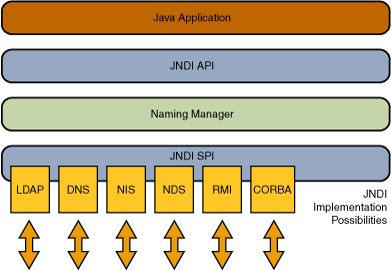
\includegraphics[scale=0.75]{images/jndiarch}
    \end{center}
    \caption{JNDI Architektur}
\end{figure}
\newline\newline
Das \gls{jndi} besteht im Grunde aus einer \gls{api} und einem \gls{spi}. Der Programmierer einer Java Applikation interagiert überwiegend mit der \gls{api}, welche
naming und directory services zur Verfügung stellt. Für spezielle Funktionalitäten sorgt das \gls{spi}, dass je nach Bedarf ein benötigtes Modul ähnlich wie ein Pluginmanager
aktiviert.\footfullcite{JNDIArchitektur} Zu den bereitgestellten Services gehören unter anderem \gls{ldap} und \gls{rmi}.\clearpage
Man betrachte nun das Logging mit Log4j:~\ref{sample-log.java}
%! Author = chaorn
%! Date = 06.01.23
\begin{lstlisting}[language=java, label={lst:sample-log.java}]
import org.apache.logging.log4j.LogManager;
import org.apache.logging.log4j.Logger;
public class MyClass {
    private static final Logger LOGGER = LogManager.getLogger();
    // ...
       LOGGER.debug("Logging in user {} with birthday {}", user.getName(), user.getBirthdayCalendar());
}
\end{lstlisting}
\captionof{lstlisting}{\texttt{sample-log.java}: Loggen mit Log4j}
